\documentclass[border=6pt]{standalone}
\usepackage{lmodern}
\usepackage[T1]{fontenc}
\usepackage{amsmath}
\usepackage{xcolor}
\usepackage{tikz}
\usetikzlibrary{arrows.meta,positioning}
\definecolor{cgray}{HTML}{8A8880}
\definecolor{cblue}{HTML}{2F7DC8}
\definecolor{camber}{HTML}{E0891E}
\definecolor{cgreen}{HTML}{4E8E2A}
\definecolor{cink}{HTML}{2B2B2B}
\tikzset{>={Stealth[length=2.2mm]}}
\def\calib{0.8,1.6,2.2,2.9,3.5,4.2,4.9,5.7,6.4,7.2,8.1,9.0}
\begin{document}
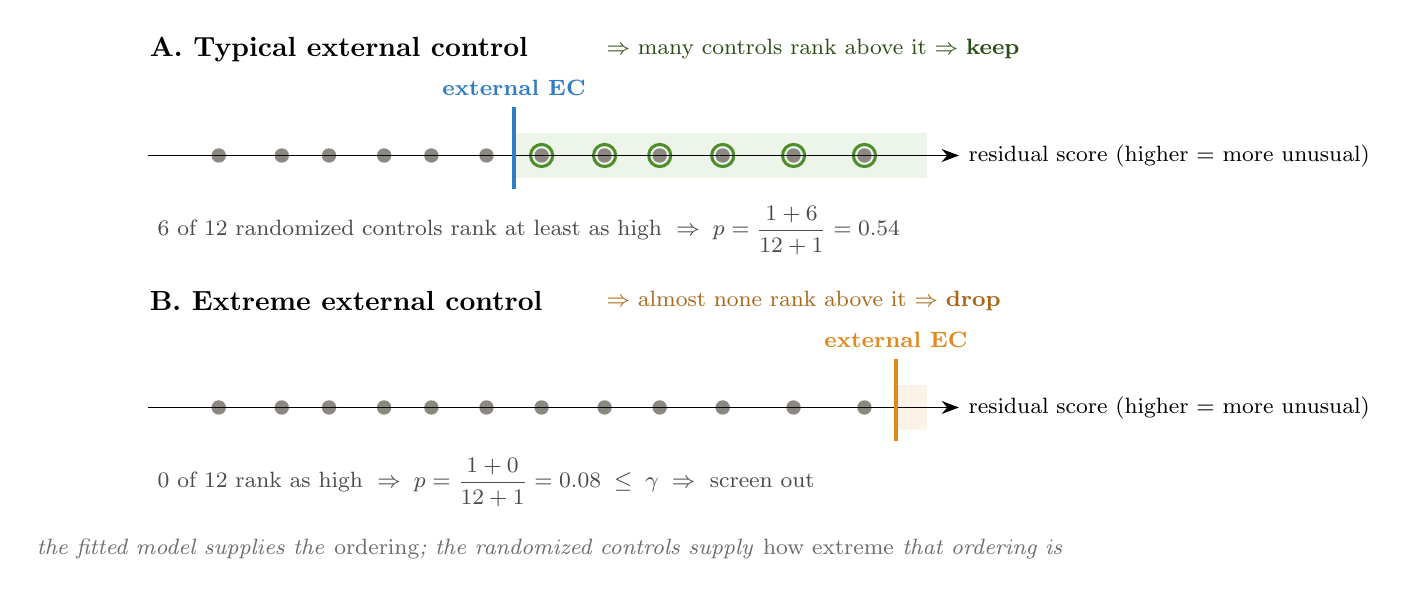
\begin{tikzpicture}[font=\small]

% ============ Panel A: typical -> keep ============
\begin{scope}
  \node[anchor=west,font=\bfseries] at (-0.2,1.35) {A. Typical external control};
  \node[anchor=west,font=\footnotesize,text=cgreen!55!black] at (5.6,1.35) {$\Rightarrow$ many controls rank above it $\Rightarrow$ \textbf{keep}};
  \fill[cgreen!10] (4.55,-0.28) rectangle (9.8,0.28);
  \foreach \x in \calib {\fill[cgray] (\x,0) circle (2.6pt);}
  \foreach \x in {4.9,5.7,6.4,7.2,8.1,9.0} {\draw[cgreen,line width=1.1pt] (\x,0) circle (4.0pt);}
  \draw[->] (-0.1,0) -- (10.2,0) node[right,font=\footnotesize]{residual score (higher $=$ more unusual)};
  \draw[cblue,line width=1.3pt] (4.55,-0.42) -- (4.55,0.62);
  \node[cblue,font=\footnotesize\bfseries,anchor=south] at (4.55,0.64) {external EC};
  \node[anchor=west,font=\footnotesize,text=cink!85] at (-0.1,-0.95)
    {$6$ of $12$ randomized controls rank at least as high $\;\Rightarrow\; p=\dfrac{1+6}{12+1}=0.54$};
\end{scope}

% ============ Panel B: extreme -> drop ============
\begin{scope}[yshift=-3.2cm]
  \node[anchor=west,font=\bfseries] at (-0.2,1.35) {B. Extreme external control};
  \node[anchor=west,font=\footnotesize,text=camber!75!black] at (5.6,1.35) {$\Rightarrow$ almost none rank above it $\Rightarrow$ \textbf{drop}};
  \fill[camber!10] (9.4,-0.28) rectangle (9.8,0.28);
  \foreach \x in \calib {\fill[cgray] (\x,0) circle (2.6pt);}
  \draw[->] (-0.1,0) -- (10.2,0) node[right,font=\footnotesize]{residual score (higher $=$ more unusual)};
  \draw[camber,line width=1.3pt] (9.4,-0.42) -- (9.4,0.62);
  \node[camber,font=\footnotesize\bfseries,anchor=south] at (9.4,0.64) {external EC};
  \node[anchor=west,font=\footnotesize,text=cink!85] at (-0.1,-0.95)
    {$0$ of $12$ rank as high $\;\Rightarrow\; p=\dfrac{1+0}{12+1}=0.08 \;\le\; \gamma \;\Rightarrow\;$ screen out};
\end{scope}

\node[anchor=north,font=\footnotesize\itshape,text=cink!70,align=center] at (5.0,-4.75)
  {the fitted model supplies the \emph{ordering}; the randomized controls supply \emph{how extreme} that ordering is};

\end{tikzpicture}
\end{document}
